\section{Phương Pháp Thực hiện}
Chương này sẽ trình bày các phương pháp và quy trình mà em sử dụng để thực hiện nghiên cứu. Đây là phần quan trọng trong đề tài, nơi mô tả cách tiến hành thu thập dữ liệu, xây dựng mô hình, đánh giá hiệu suất và ứng dụng thực tế của công nghệ OCR trong việc nhận dạng và xử lý hóa đơn.

Dưới đây là các bước trình bày chi tiết:
\begin{enumerate}
    \item \textbf{Phầm mềm và công cụ hỗ trợ:} Trình bày các phầm mềm và công cụ cho quá trình chuẩn bị dữ liệu, xây dựng và huấn luyện mô hình.
    \item \textbf{Lựa chọn loại hóa đơn:} Để định rõ phạm vi nghiên cứu, em sẽ lựa chọn một loại hóa đơn cụ thể để tập trung trong đề tài. Việc này giúp xác định rõ mục tiêu và hướng đi của phần còn lại trong chương này.
    \item \textbf{Thu thập dữ liệu:} Mô tả quy trình thu thập dữ liệu, bao gồm cách chọn các hình ảnh hóa đơn, cách đảm bảo tính đa dạng và độ phủ của dữ liệu, và việc chuẩn bị dữ liệu cho quá trình huấn luyện và kiểm tra mô hình.
    \item \textbf{Xây dựng mô hình OCR}: Trong phần này, sẽ mô tả quá trình xây dựng mô hình nhận diện, nhận dạng OCR và Trích xuất thông tin chính. Giới thiệu mạng nơ-ron học sâu và cấu trúc các mô hình, thiết lập các lớp, tham số và hàm kích hoạt.
    \item \textbf{Huấn luyện và tinh chỉnh:} Mô tả cách huấn luyện mô hình trên tập dữ liệu đã thu thập. Điều chỉnh tham số, tối ưu hóa và giải quyết vấn đề overfitting hoặc underfitting.

\end{enumerate}

Chương "Phương pháp thực hiện" là nền tảng quan trọng cho việc thực hiện nghiên cứu, giúp định hình cách tiến hành các bước quan trọng trong đề tài "Nghiên cứu ứng dụng công nghệ OCR nhận dạng hóa đơn".

\subsection{Phầm mềm và công cụ hỗ trợ}
\subsubsection{Google Colab}
Google Colab (viết tắt của Google Colaboratory) là một dịch vụ miễn phí của Google cho phép thực hiện và chia sẻ các tệp notebook Jupyter, cũng như code Python. Nó là một môi trường trực tuyến, cho phép người dùng viết và chạy code Python một cách trực toeép trên trình duyệt web mà không cần cài đặt bất kỳ môi trường phát triển nào trên máy tính.

Colab cung cấp sử dụng miễn phí cho CPU, GPU và RAM để người dùng có thể thực hiện các nhiệm vụ tính toán phức tạp mà không cần phải mua hoặc cấu hình phần cứng riêng. Colab còn được tích hợp sẵn với nhiều thư viện phổ biến cho khoa học dữ liệu, học máy và xử lý ảnh, giúp dễ dàng tiến hành các tác vụ phức tạp. Có thể tạo notebook Jupyter, trong đó bạn có thể viết code Python từng cell và thực thi chúng một cách tương tác. Điều này rất hữu ích cho việc thử nghiệm, phân tích dữ liệu và xây dựng mô hình máy học.

Colab có thể chia sẻ notebook của mình với người khác thông qua liên kết. Người khác có thể xem và chỉnh sửa notebook hoặc thậm chí làm việc chung với nhau trên cùng một notebook. Có thể lưu notebook và dữ liệu của mình trực tiếp vào Google Drive để truy cập dễ dàng và chia sẻ với các thiết bị khác.

Google Colab thường được sử dụng trong việc học, nghiên cứu và phát triển các dự án liên quan đến khoa học dữ liệu, học máy và trí tuệ nhân tạo mà không cần đầu tư nhiều vào cấu hình phần cứng.

\subsubsection{PaddleOCR}
PaddleOCR là một dự án mã nguồn mở do PaddlePaddle phát triển, nhằm cung cấp một giải pháp toàn diện cho các nhiệm vụ liên quan đến xử lý ảnh và văn bản, bao gồm cả nhận dạng ký tự, nhận dạng văn bản và các tác vụ liên quan đến OCR. Dự án này được xây dựng trên cơ sở của các mô hình học sâu và sử dụng các thuật toán tiên tiến để giải quyết các thách thức trong việc xử lý ảnh và văn bản.

PaddleOCR hỗ trợ nhiều tác vụ liên quan đến OCR như nhận dạng ký tự, nhận dạng văn bản và phân loại chữ viết tay. Có thể được đào tạo và sử dụng cho nhiều ngôn ngữ khác nhau, giúp phát triển ứng dụng OCR toàn cầu. Người dùng có thể tùy chỉnh và đào tạo lại các mô hình của PaddleOCR cho phù hợp với nhu cầu cụ thể của dự án.

PaddleOCR có thể hoạt động trên nhiều nền tảng khác nhau, bao gồm máy tính cá nhân, máy chủ và các môi trường đám mây. Dự án cung cấp một loạt các mô hình học sâu đã được đào tạo trước để giúp giải quyết các vấn đề liên quan đến xử lý ảnh và văn bản.

Dự án được tối ưu hóa để đạt hiệu suất cao và đáp ứng yêu cầu xử lý ảnh và văn bản trong thời gian thực.

Hơn nữa PaddleOCR là một dự án mã nguồn mở và có cộng đồng hỗ trợ sẵn sàng chia sẻ kiến thức, giải đáp thắc mắc và cùng nhau phát triển.

Tóm lại, cung cấp một giải pháp mạnh mẽ và linh hoạt cho các ứng dụng liên quan đến xử lý ảnh và văn bản, đặc biệt là trong lĩnh vực OCR. Điều này giúp đơn giản hóa và tối ưu hóa quá trình xây dựng hệ thống nhận dạng văn bản và thông tin từ các hình ảnh hóa đơn và tài liệu khác.

\subsubsection{PPOCRLabel}
PPOCRLabel là một công cụ hỗ trợ trong lĩnh vực xử lý ảnh và trí tuệ nhân tạo, được sử dụng để thực hiện công việc nhận dạng và đánh dấu vùng chứa văn bản trên ảnh. Đây là một dự án mã nguồn mở của PaddlePaddle, một thư viện học máy phát triển bởi Baidu. PaddleOCR nhằm mục tiêu xây dựng các mô hình nhận dạng ký tự trên ảnh với hiệu suất cao.

PPOCRLabel được tạo ra để hỗ trợ quá trình chuẩn bị dữ liệu cho việc huấn luyện mô hình nhận dạng văn bản. Việc chuẩn bị dữ liệu là một bước quan trọng trong quá trình phát triển mô hình học máy, và công cụ như PPOCRLabel giúp đơn giản hóa và tăng cường hiệu suất của quá trình này. Dưới đây là một số tính năng chính của PPOCRLabel \cite{ppocrlabel}:
\begin{enumerate}
    \item \textbf{Labeling vùng chứa văn bản:} PPOCRLabel cho phép người dùng vẽ các hộp giới hạn xung quanh các vùng chứa văn bản trên ảnh để đánh dấu vị trí của văn bản cần nhận dạng.
    \item \textbf{Labeling trích xuất từ khóa:} Người dùng có thể gán nhãn thông tin từ khóa để cho bài toán trích xuất thông tin chính.
    \item \textbf{Gắn nhãn văn bản:} Người dùng có thể gắn nhãn văn bản được nhận dạng trong các hộp giới hạn để cho biết nội dung của văn bản đó.
    \item \textbf{Chú thích cho bảng:} PPOCRLabel cung cấp cho người dùng chức năng chú thích bảng nhằm mục đích bóc tách cấu trúc của bảng dưới dạng hình ảnh và chuyển sang định dạng Excel
    \item \textbf{Chỉnh sửa và xem trước:} PPOCRLabel cung cấp giao diện để chỉnh sửa và xem trước dữ liệu đã được đánh dấu trên ảnh, đảm bảo rằng dữ liệu được chuẩn bị chính xác trước khi sử dụng để huấn luyện mô hình.
    \item \textbf{Xuất dữ liệu:} Sau khi hoàn thành việc đánh dấu và chuẩn bị dữ liệu, PPOCRLabel cho phép bạn xuất dữ liệu trong các định dạng phổ biến để sử dụng trong quá trình huấn luyện mô hình.
    \item \textbf{Tích hợp với PaddleOCR:} PPOCRLabel có thể liên kết với dự án PaddleOCR để tiện lợi trong việc sử dụng dữ liệu đã được chuẩn bị để huấn luyện các mô hình nhận dạng văn bản.
\end{enumerate}

PPOCRLabel là một công cụ cực kỳ hữu ích trong quá trình chuẩn bị dữ liệu cho việc huấn luyện mô hình liên quan đến OCR, giúp tăng cường hiệu suất và chính xác của mô hình cuối cùng.

\subsection{Lựa chọn hóa đơn}
Trong phần này, em xác định loại hóa đơn mà nghiên cứu sẽ tập trung nhằm mục tiêu ứng dụng công nghệ OCR trong việc nhận dạng và trích xuất thông tin. Loại hóa đơn được chọn là hóa đơn bán hàng ở cửa hàng tiện lợi và siêu thị, là một phần quan trọng của cuộc sống hàng ngày và có sự đại diện cho nhiều thông tin đa dạng cần được xử lý.

Hóa đơn bán hàng cửa hàng tiện lợi và siêu thị được lựa chọn vì nó thường chứa các thông tin cần thiết như địa chỉ, ngày mua, sản phẩm, số lượng, cũng như các khoản phí.\ldots Loại hóa đơn này thường đa dạng về cấu trúc và kiểu dáng, bao gồm vùng văn bản in và cả phần hình ảnh với các dữ liệu chú thích. Do đó, ứng dụng công nghệ OCR để tự động nhận dạng và trích xuất thông tin từ loại hóa đơn này đem lại giá trị thực tiễn và hứa hẹn trong việc tối ưu hóa quá trình xử lý hóa đơn và quản lý tài liệu.

Để thực hiện đề tài này em sử dụng mẫu hóa đơn của cửa hàng tiện lợi Okono và VinMart (Hình \ref{fig9-okono-vincom}) để thực hiện trích xuất thông tin.

\begin{figure}
    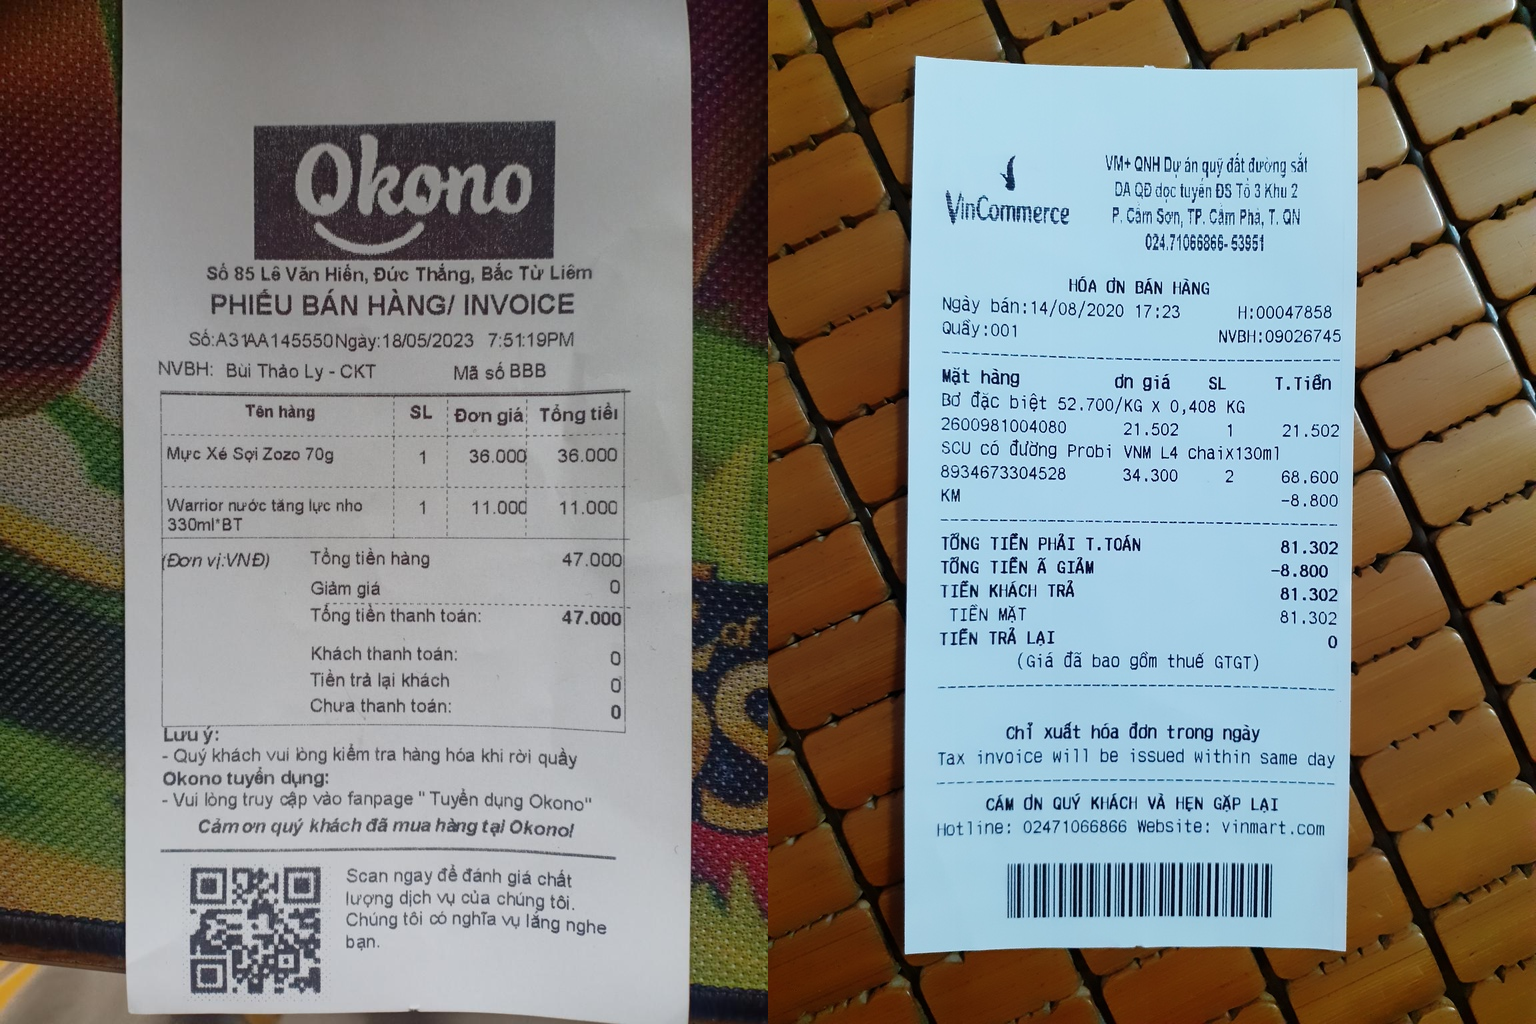
\includegraphics[scale=0.28]{images/okono-vincom.png}
    \centering
    \caption{Hóa đơn Okono(trái) và VinCommerce(phải)}
    \label{fig9-okono-vincom}
\end{figure}

Qua việc tập trung vào loại hóa đơn bán hàng cửa hàng tiện lợi và siêu thị, mong muốn thực hiện một nghiên cứu chi tiết về cách ứng dụng công nghệ OCR vào việc nhận dạng và xử lý dữ liệu từ hóa đơn trong ngữ cảnh thực tế.

\subsection{Thu thập và chuẩn bị dữ liệu}
Thu thập và chuẩn bị dữ liệu cho nhiệm vụ Nhận dạng ký tự trên ảnh là một bước quan trọng để đảm bảo rằng mô hình OCR hoạt động tốt trên các dữ liệu thực tế. Trong phần này, em sẽ trình bày quá trình thu thập và xử lý dữ liệu hình ảnh của hóa đơn hàng cửa hàng tiện lợi và siêu thị. Việc thu thập dữ liệu là bước quan trọng để xây dựng và huấn luyện mô hình nhận dạng OCR. Tùy với nhiệm vụ khác nhau trong OCR ta có cách chuẩn bị dữ liệu khác nhau.

Về thu thập dữ liệu em sử dụng hóa đơn Okono thu thập từ cửa hàng tiện lợi Okono ở 85 Lê Văn Hiến, và hóa đơn VinCommerce em đã thu thập từ bộ dataset của cuộc thi \textbf{Mobile-Captured Image Document Recognition for Vietnamese Receipts (MC-OCR) - Legacy}


% \begin{center}
%     \begin{tabular}{ |c|c|c| } 
%      \hline
%            & Tổng số mẫu \\ 
%      \hline
%      Train & 1.000.472 \\ 
%      \hline
%      Valid & 230.024 \\ 
%      \hline
%     \end{tabular}
% \end{center}

% \begin{figure}
%     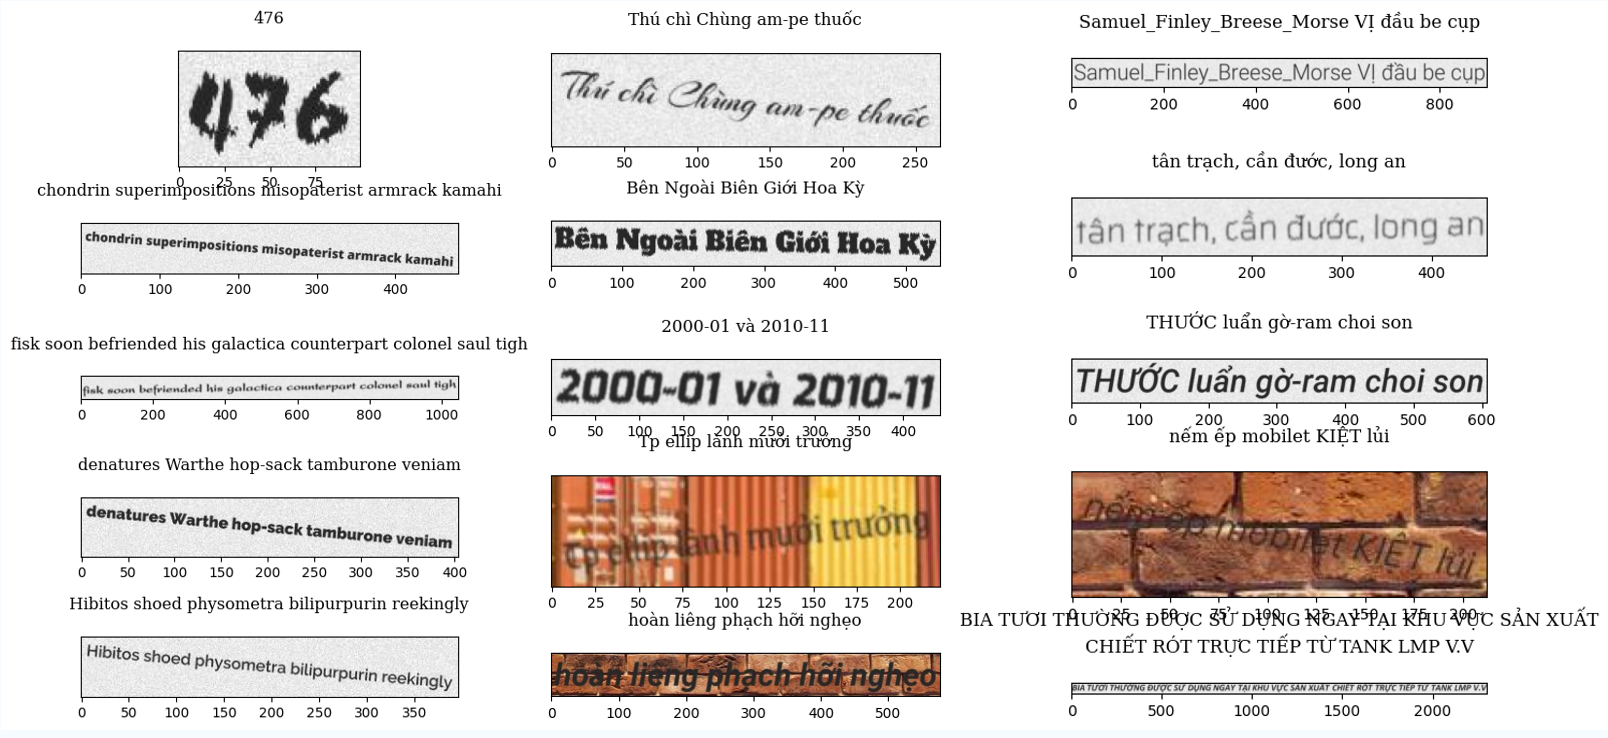
\includegraphics[scale=0.36]{images/data-text-recognition.png}
%     \centering
%     \caption{Dữ liệu cho nhận dạng văn bản}
% \end{figure}

\subsection{Xây dựng hệ thống}
Để xây dựng một hệ thống OCR cho nhiệm vụ nhận diện hóa đơn đây là một quá trình phức tạp đòi hỏi sự kết hợp giữa nhiều nhiệm vụ khác nhau để đảm bảo hiệu suất và chất lượng của quá trình nhận dạng như Phát hiện vùng văn bản, Nhận dạng văn bản và Hiểu tài liệu(Document Understanding)

\subsubsection{Phát hiện văn bản}
Ở đề tài này em sử dụng DBNet \cite{liao2019realtime} (Differentiable Binarization Network), đây là một mô hình mạng nơ-ron sử dụng trong lĩnh vực phát hiện văn bản. Phương pháp này tập trung vào vấn đề chuyển đổi hình ảnh văn bản đa dạng thành hình ảnh nhị phân, đồng thời huấn luyện mạng theo cách có thể tối ưu hóa quá trình này. Phương pháp nhị phân hoá khác biệt của DBNet cho phép giữ lại thông tin quan trọng trong hình ảnh và loại bỏ thông tin không cần thiết, giúp cải thiện độ chính xác của quá trình nhận dạng ký tự.

DB là một thuật toán dựa trên phân đoạn để phát hiện văn bản, sử dụng một mô-đun Nhị phân hóa Ngưỡng Khả vi (DB) khác biệt để phân biệt vùng văn bản khỏi nền với một ngưỡng động.

\begin{figure}[h]
    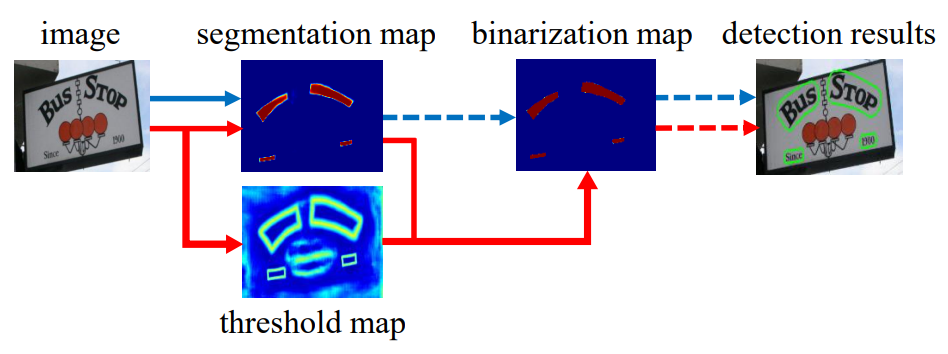
\includegraphics[scale=0.5]{images/tradition-db-pipeline.png}
    \centering
    \caption{Pipeline truyền thống (luồng màu xanh) và pipeline của DB (luồng màu đỏ) }
    \label{}
\end{figure}

Những mũi tên màu xanh trong hình minh họa cho quy trình của các thuật toán phát hiện văn bản dựa trên phân đoạn thông thường. Loại phương pháp này sử dụng một ngưỡng cố định để tạo ra bản đồ phân đoạn nhị phân sau khi phân đoạn, sau đó áp dụng các thuật toán heuristics như gom cụm pixel để có được vùng văn bản.
Những mũi tên màu đỏ trong hình minh họa cho luồng của thuật toán DB. Sự khác biệt lớn nhất so với các giải pháp thông thường là DB có một bản đồ ngưỡng, và nó sẽ dự đoán ngưỡng tại mỗi điểm pixel của hình ảnh thông qua mạng neural, thay vì chỉ định một giá trị cố định. Do đó, nó có thể phân biệt tốt hơn giữa nền và vùng văn bản.

Thuật toán DB có những ưu điểm sau:
\begin{enumerate}
    \item Cấu trúc thuật toán đơn giản và không cần xử lý sau quá trình tính toán phức tạp
    \item Dữ liệu nguồn mở của nó có độ chính xác và hiệu suất tốt
\end{enumerate}
Sau khi có bản đồ xác suất, thuật toán truyền thống dựa trên phân đoạn hình ảnh sẽ đặt tất cả các điểm ảnh có giá trị thấp hơn ngưỡng t thành 0 và ngược lại thành 1. Công thức là: 
$$
B_{i, j} = \begin{cases}
    1, \text{if } P_{i, j} \geq t, \\
    0, \text{otherwise}
\end{cases} 
$$

Nhưng phương pháp nhị phân tiêu chuẩn không có khả năng khác biệt, từ đó khiến mạng không thể được huấn luyện theo kiểu end-to-end (tức là không thể tích hợp vào quá trình lan truyền ngược). Để giải quyết vấn đề này, thuật toán DB sử dụng Differentiable Binarization, giúp xấp xỉ step function của phương pháp nhị phân tiêu chuẩn. Nó sử dụng công thức khác:
\[
    \hat{B} = \frac{1}{1+e^{-k(P_{i, j} - T_{i, j})}}    
\]

Ở trên, $P$ đề cập đến bản đồ xác suất, $T$ đề cập đến bản đồ ngưỡng, và $k$ là hệ số tăng được thiết lập là 50 dưới một quy tắc thực tế trong thí nghiệm. Hình \ref{fig11}(a) dưới đây cho thấy sự khác biệt giữa phương pháp nhị phân tiêu chuẩn và phân đoạn khác biệt.

Khi sử dụng hàm mất mát cross-entropy, mất mát của các mẫu dương và mẫu âm lần lượt là $l_+$ và $l_-$:
\[
    l_+ = -\log(\frac{1}{1+e^{-k(P_{i, j}-T_{i, j})}})
\]
\[
    l_- = -\log(1 - \frac{1}{1 + e^{-k(P_{i, j} - T_{i, j})}})
\]

Nhập $x$ vào để lấy đạo hàm riêng có thể dẫn đến:
\[
    \frac{\delta l_+}{\delta x} = -kf(x)e^{-kx}
\]
\[
    \frac{\delta l_-}{\delta x} = -kf(x)   
\]

Có thể thấy rằng hệ số tăng sẽ làm phình to độ dốc của dự đoán lỗi, từ đó tối ưu hóa mô hình để đạt được kết quả tốt hơn. Trong Hình \ref{fig11}(b), phần của $x < 0$ đại diện cho trường hợp mẫu tích cực được dự đoán thành mẫu tiêu cực. Có thể thấy rằng hệ số tăng k làm phình to độ dốc. Hình \ref{fig11}(c) hiển thị $x > 0$, đề cập đến trường hợp mẫu tiêu cực được dự đoán thành mẫu tích cực, và độ dốc cũng được phình to.

\begin{figure}[h]
    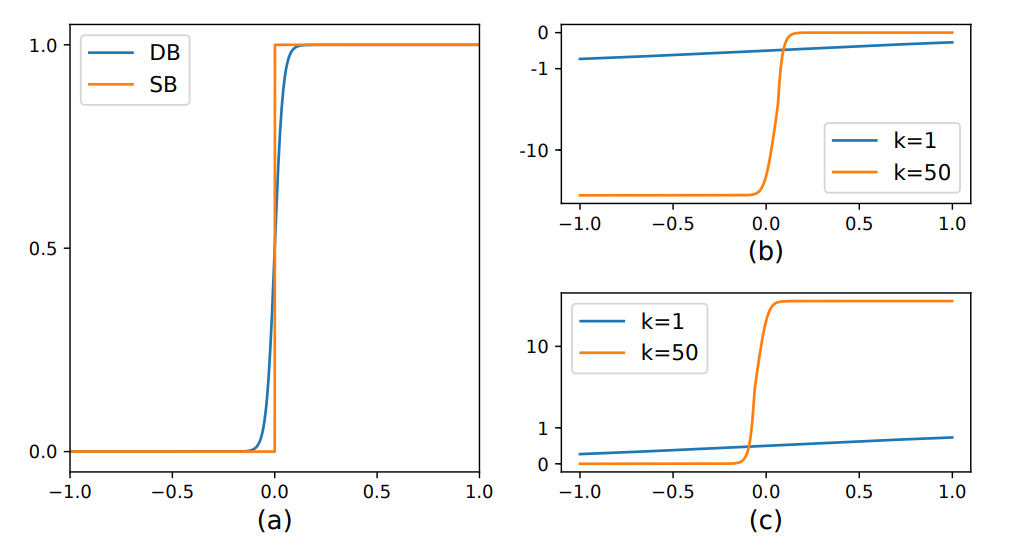
\includegraphics[scale=0.5]{images/derivative-DB.png}
    \centering
    \caption{Minh họa về phân đoạn khác biệt và đạo hàm của nó. (a) So sánh số liệu giữa phương pháp nhị phân tiêu chuẩn (SB) và phân đoạn khác biệt (DB). (b) Đạo hàm của $l_+$. (c) Đạo hàm của $l_-$. \cite{liao2019realtime}}
    \label{fig11}
\end{figure}

\begin{figure}[h]
    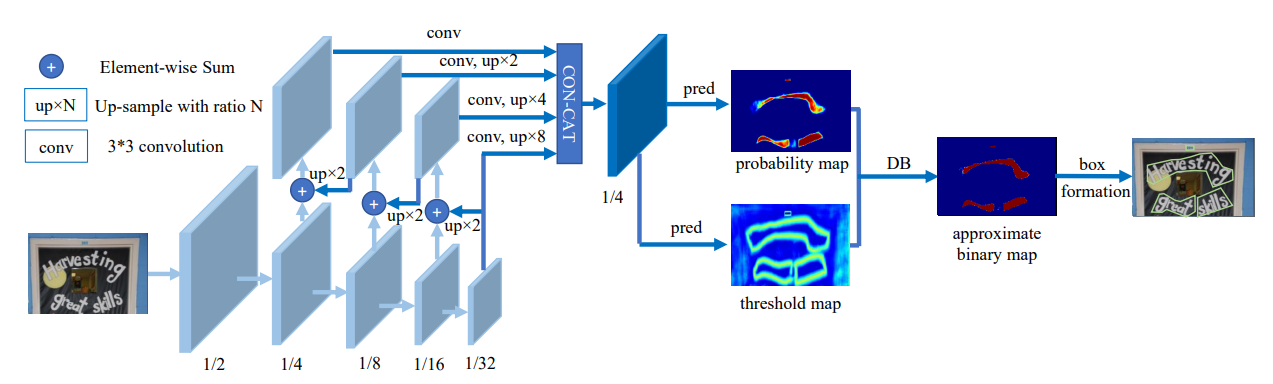
\includegraphics[scale=0.45]{images/architecture-db.png}
    \centering
    \caption{Kiến trúc của phương pháp DB}
    \label{fig12}
\end{figure}

Cấu trúc tổng quan của thuật toán DB (Hình \ref{fig12}), các đặc điểm của hình ảnh đầu vào được trích xuất thông qua mạng Backbone và FPN, sau đó chúng được nối liền để tạo ra một đặc điểm có kích thước là một phần tư của hình ảnh gốc. Sau đó, lớp tích chập được sử dụng để tạo ra bản đồ xác suất dự đoán và bản đồ ngưỡng, và sau đó tạo ra đường viền qua quá trình xử lý sau cùng của DB.

\subsubsection{Nhận dạng văn bản}
\subsubsection{Hiểu tài liệu}

